\section{melcomp\_1}

In melcomp\_1 I set out with three questions:
\begin{enumerate}
\item Considering only daylight spectra (excluding reflective surfaces for now), can a melanopic signal measure the chromaticity of daylight? % more precisely? as well as? in the same league?
\item Now considering also object reflectances, does a melanopic signal provide a means of calculating a sign and weight of shift required to counteract the chromatic shift induced upon objects by a change in daylight conditions?
\item Are there objects, or luminance levels, or daylight chromaticities for which the melanopic signal is particularly effective or ineffective at performing the above task?
\end{enumerate}

Foundational data consisting of 
the Granada daylight dataset 
\citep{hernandez-andres_color_2001}\footnote{Data: \url{http://colorimaginglab.ugr.es/pages/Data\#__doku_granada_daylight_spectral_database}},
the Stockman-Sharpe 10$^{\circ}$ cone fundamentals 
\citep{stockman_spectral_2000,stockman_spectral_1999}
(aka the CIE 2006 10$^{\circ}$ cone fundamental sensitivity functions \cite{cie_cie_2006})\footnote{Available as `T\_cones\_ss10' in \gls{PTB}.},
the melanopsin fundamental of \citet{lucas_measuring_2014}\footnote{Available as `T\_melanopsin' in \gls{PTB}.},
and a subset\footnote{For these computations 11 surfaces were chosen from the Vrhel dataset, with a roughly even representation of skin tones, fruit, and vegetable/greenery.} 
of the reflectances of \citet{vrhel_measurement_1994}\footnote{Available as `sur\_vrhel' in \gls{PTB}.}
were used.
% Many MANY other things were considered, but I think perhaps I'll summarise those elsewhere

Initial computations considered the illuminants alone, without considering the interaction with surface reflectances (as per question 1). However, to avoid repeating text and figures here I shall discuss this approach alongside that taken to answer question 2. Figures in this section use red for illuminant only chromaticities and grey for surfaces. 

Tristimulus values $[L,M,S]$ and analogous melanopic values $I$ (as per standard tristumulus values but using the melanopsin fundamental) were computed as per eq X %
for each illuminant within the Granada dataset, and for each surface under each illuminant. A real-world version of the first set of values would be to measure a spectralon tile (or other uniformally reflective surface) under each daylight condition. \gls{MB} chromaticity co-ordinates were calculated, again for both illuminant alone and for each surface under each illuminant, as per equation X. %
The \gls{MB} chromaticities are plotted in Figure \ref{fig:MB}. Three-dimensional plots were made to display $l_{\text{MB}}$ against $s_{\text{MB}}$ against $[L,M,S,I]$ in turn. Each plot is shown in Figure \ref{fig:level1}. 

\begin{figure}[htbp]
    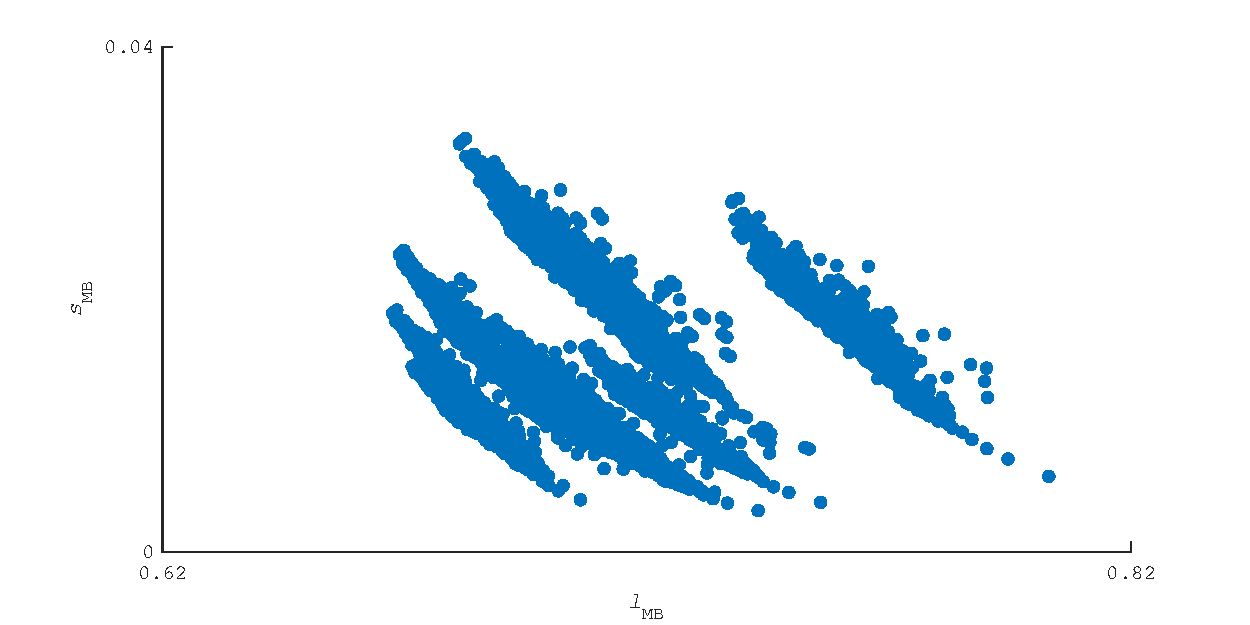
\includegraphics[max width=\textwidth]{figs/comp/melcomp_1/BasicMB.pdf}
    \caption{\gls{MB} chromaticities for 12 reflectances under 2600 daylight illuminants (grey-centred circles with colours denoting different surfaces, colours not linked to real colours, solely for visualisation), and chromaticities for illuminants alone (red-centred, black bordered circled).}
    \label{fig:MB}
\end{figure} 

\begin{figure}[htbp]
    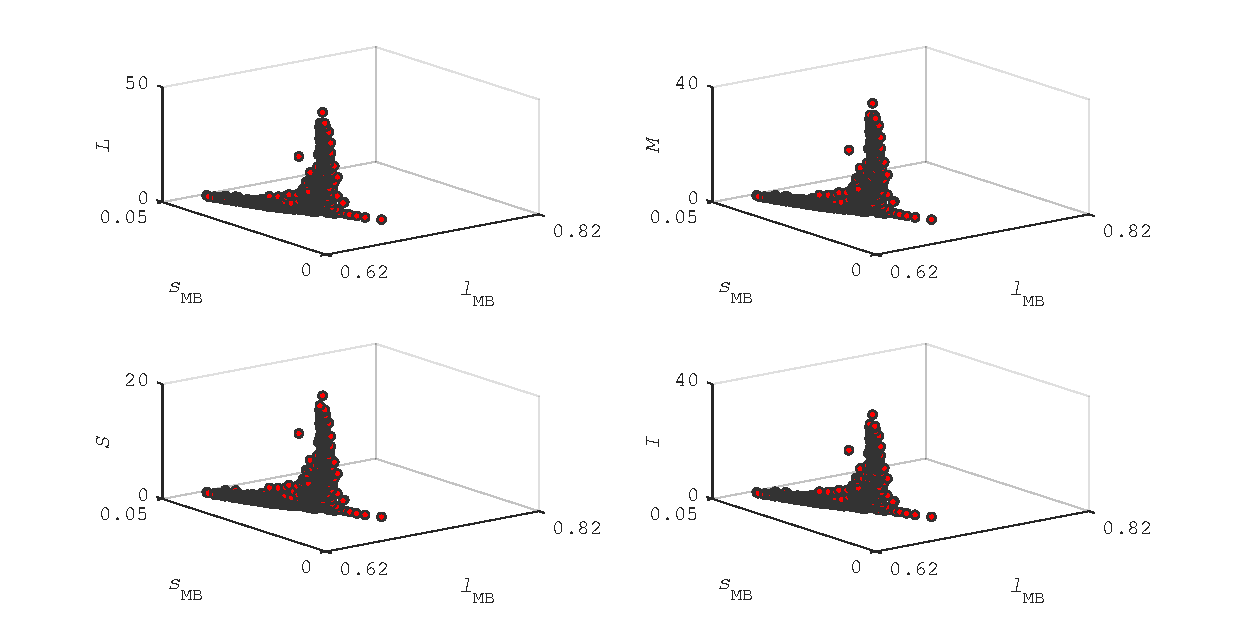
\includegraphics[max width=\textwidth]{figs/comp/melcomp_1/level1sigspredictingColorimetry.pdf}
    \caption{\gls{MB} chromaticity diagram on the horizontal plane ($l_{\text{MB}}$ against $s_{\text{MB}}$), with $[L,M,S,I]$ plotted in turn on the z-axis, for the illuminants of the Granada dataset, and a subset of the Vrhel reflectances. Red points indicate signals computed directly from the spectral power distribution, grey points represent values of computed colorimetry for objects under illuminants. Note - vertical axes rescaled per plot. For the red (illuminant only) points, in each graph the trend from left-to-right above is to start low with a gradual increase before fairly rapidly going vertical. Though hard to see here, the grey points follow the same trend, but on a surface-by-surface level.}
    \label{fig:level1}
\end{figure} 

From Figure \ref{fig:level1}, it can be seen that although there exists some relationship between the chromaticity values of the illuminants and the $[L,M,S,I]$ values, it does not appear as though one could be used to reliably predict the other. All that can be gained from this relationship is the understanding that if the $[L,M,S,I]$ value is above a certain threshold, it is likely to be in a group with a low $s_{\text{MB}}$ and high $l_{\text{MB}}$ value. The real-world correlate of this is - \textit{if the daylight is bright enough, I can be fairly confident that the chromaticity of light will be relatively warm in colour.} This is as expected, since the brightest daylight conditions are likely to be those with unobstructed direct sunlight, which is warmer in \gls{CCT} than illumination provided by the blue sky. This relationship seems relatively weak however, and could not be used to accurately predict the chromaticity of an illuminant. 

The answer to the first question set out for the script then, is that a melanopic signal cannot predict chromaticity (though neither can any other single signal). In regard to the second question, whilst a similar relationship is seen, it is on a surface-by-surface level (each group of points representing a single surface shows a similar trend to that highlighted in red for the illuminant-only points, but each group is distinct, though often overlapping, from others). The effect of this would be that for a random surface under a random illuminant, any of the $[L,M,S,I]$ values would do a poor job of predicting the chromaticity of the illuminant. The melanopsin-based value ($I$) certainly does not do a markedly better job than other values.

\begin{figure}[htbp]
    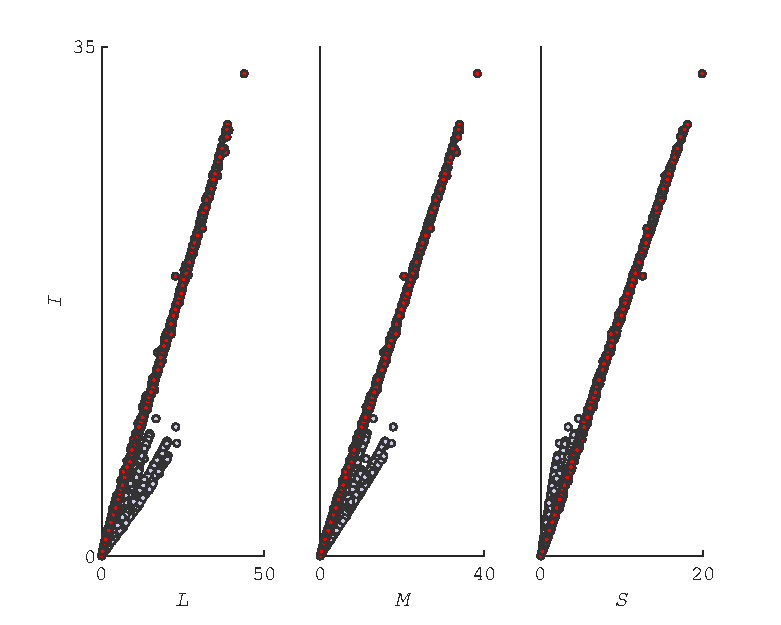
\includegraphics[max width=\textwidth]{figs/comp/melcomp_1/correlationBetweenLevel1Sigs.pdf}
    \caption{The relationship between melanopic power (analogous to a tristimulus value but calculated using the spectral sensitivity of melanopsin). Red points indicate signals computed directly from the spectral power distribution, grey points represent values of computed colorimetry for objects under illuminants.  The traditional tristimulus values show a very strong correlation for illuminant-only values. It is not particularly easy to see here, but each surface is represented by a roughly straight line of grey points at slightly different angles.}
    \label{fig:tristimCorrelation}
\end{figure} 

It should be noted that there was very high correlation between each signal. This is shown in Figure \ref{fig:tristimCorrelation} and the correlation table below. This can be considered as corresponding to the high importance of the first principal component of the spectral measurements in this dataset. Put another way, a sensor with almost any spectral sensitivity could be used to estimate the general magnitude of the daylight. I shall return to the discussion of principal components when discussing melcomp\_3.

\begin{minipage}{\linewidth}
\begin{lstlisting}
corr(LMSI)
    1.0000    1.0000    0.9993    0.9998
    1.0000    1.0000    0.9995    0.9999
    0.9993    0.9995    1.0000    0.9999
    0.9998    0.9999    0.9999    1.0000
\end{lstlisting}
\end{minipage}

\bigskip

Following this, similar plots were made which plotted $l_{\text{MB}}$ against $s_{\text{MB}}$ as before, but now plotted the various combinations of $[L,M,S,I]$, created by considering one signal over another (e.g. $L/M$), on the z-axis. These plots are shown in Figure \ref{fig:allComboSignals}. Following the terminology of \citet{barrionuevo_contributions_2014} I shall refer to $[L,M,S,I]$ as `first level signals' and these derived signals as `second level signals'. The twelve plots created all showed clear and relatively simple relationships between chromaticity and these new derived signals, at least for the illuminant-only values. Again, a similar trend was seen for each individual surface, but once surfaces were included any overall trend broke down into small replicants of the overall trend.
% This might end up putting a single line on a page. Check before submitting

\clearpage
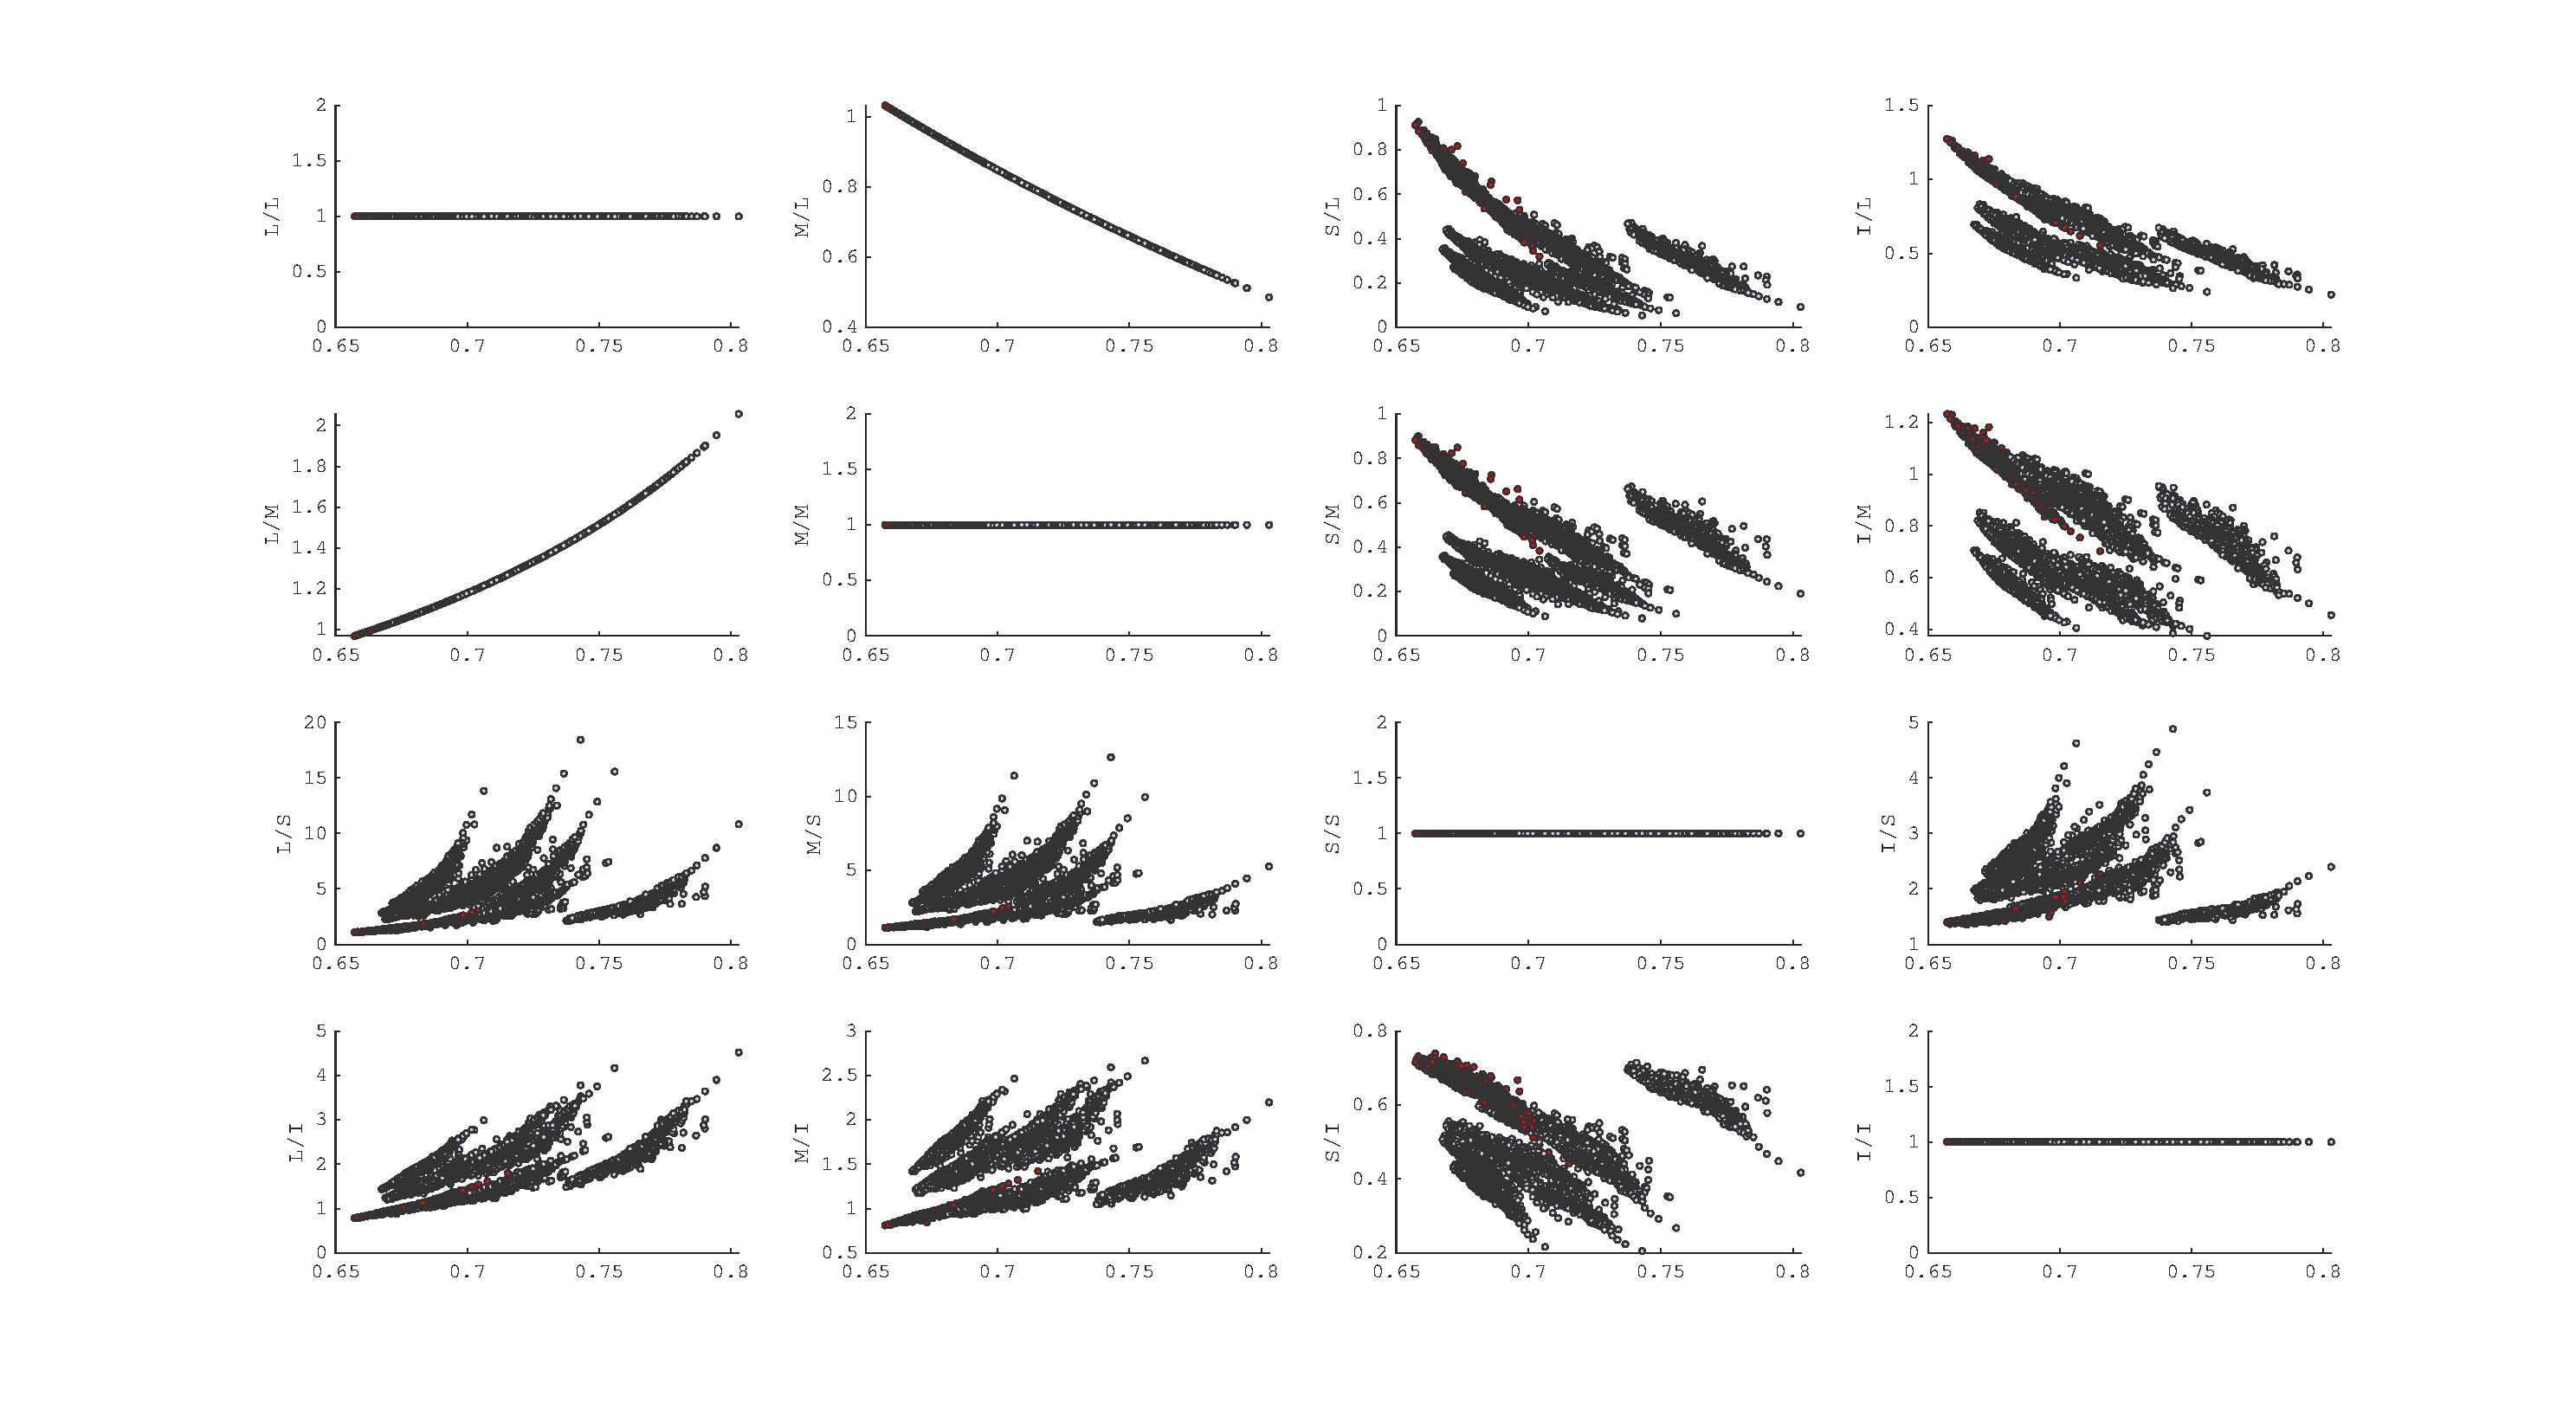
\includepdf[pages=-,rotate=90, offset=75 -75]{figs/comp/melcomp_1/allComboSignals.pdf}
\begin{figure}[h!]
    \caption{Relationship between chromaticity and second level signals. Plotted on the x-axis here is $l_{\text{MB}}$, with second level signals on the apparent y-axis. During analysis these plots were three dimensional, with the apparent y-axis being a z-axis and the x-axis joined by a y-axis of $s_{\text{MB}}$. As before, red points indicate signals computed directly from the spectral power distribution, grey points represent values of computed colorimetry for objects under illuminants. It can be seen that on a per object basis (incl. no object) there is good correlation between all of the above signals (though often it is non-linear).}
    % See gifs online at...
    \label{fig:allComboSignals}
\end{figure} 
%\clearpage
% does it look weird if this doesn't spread over a double?

For many of these signals however, such relationships are to be expected\footnote{My thanks go to Manuel Spitschan for convincing me of this point.}. For example, a relationship between $l_{\text{MB}}$ and $L/M$ should be expected, since $l_{\text{MB}}$ is defined as the sum of weighted components of $L$ and $M$. To confirm this, a null condition was performed, where $[L,M,S,I]$ was replaced by randomly generated values, and the second level signals were generated as before. The results can be seen in Figure \ref{fig:allComboSignals_rand}. Relationships between secondary signals derived from $L$, $M$ or $S$ signals still showed correlations with chromaticity (albeit now points fell on a plane, instead of a line), whereas signals with a $I$ component showed only minimal coherence, forming a noisy cloud in three-dimensional space. This implies that should the melanopic signals correlate with chromaticity, that this is not simply a computational artefact of the way in which chromaticity is calculated.

\clearpage
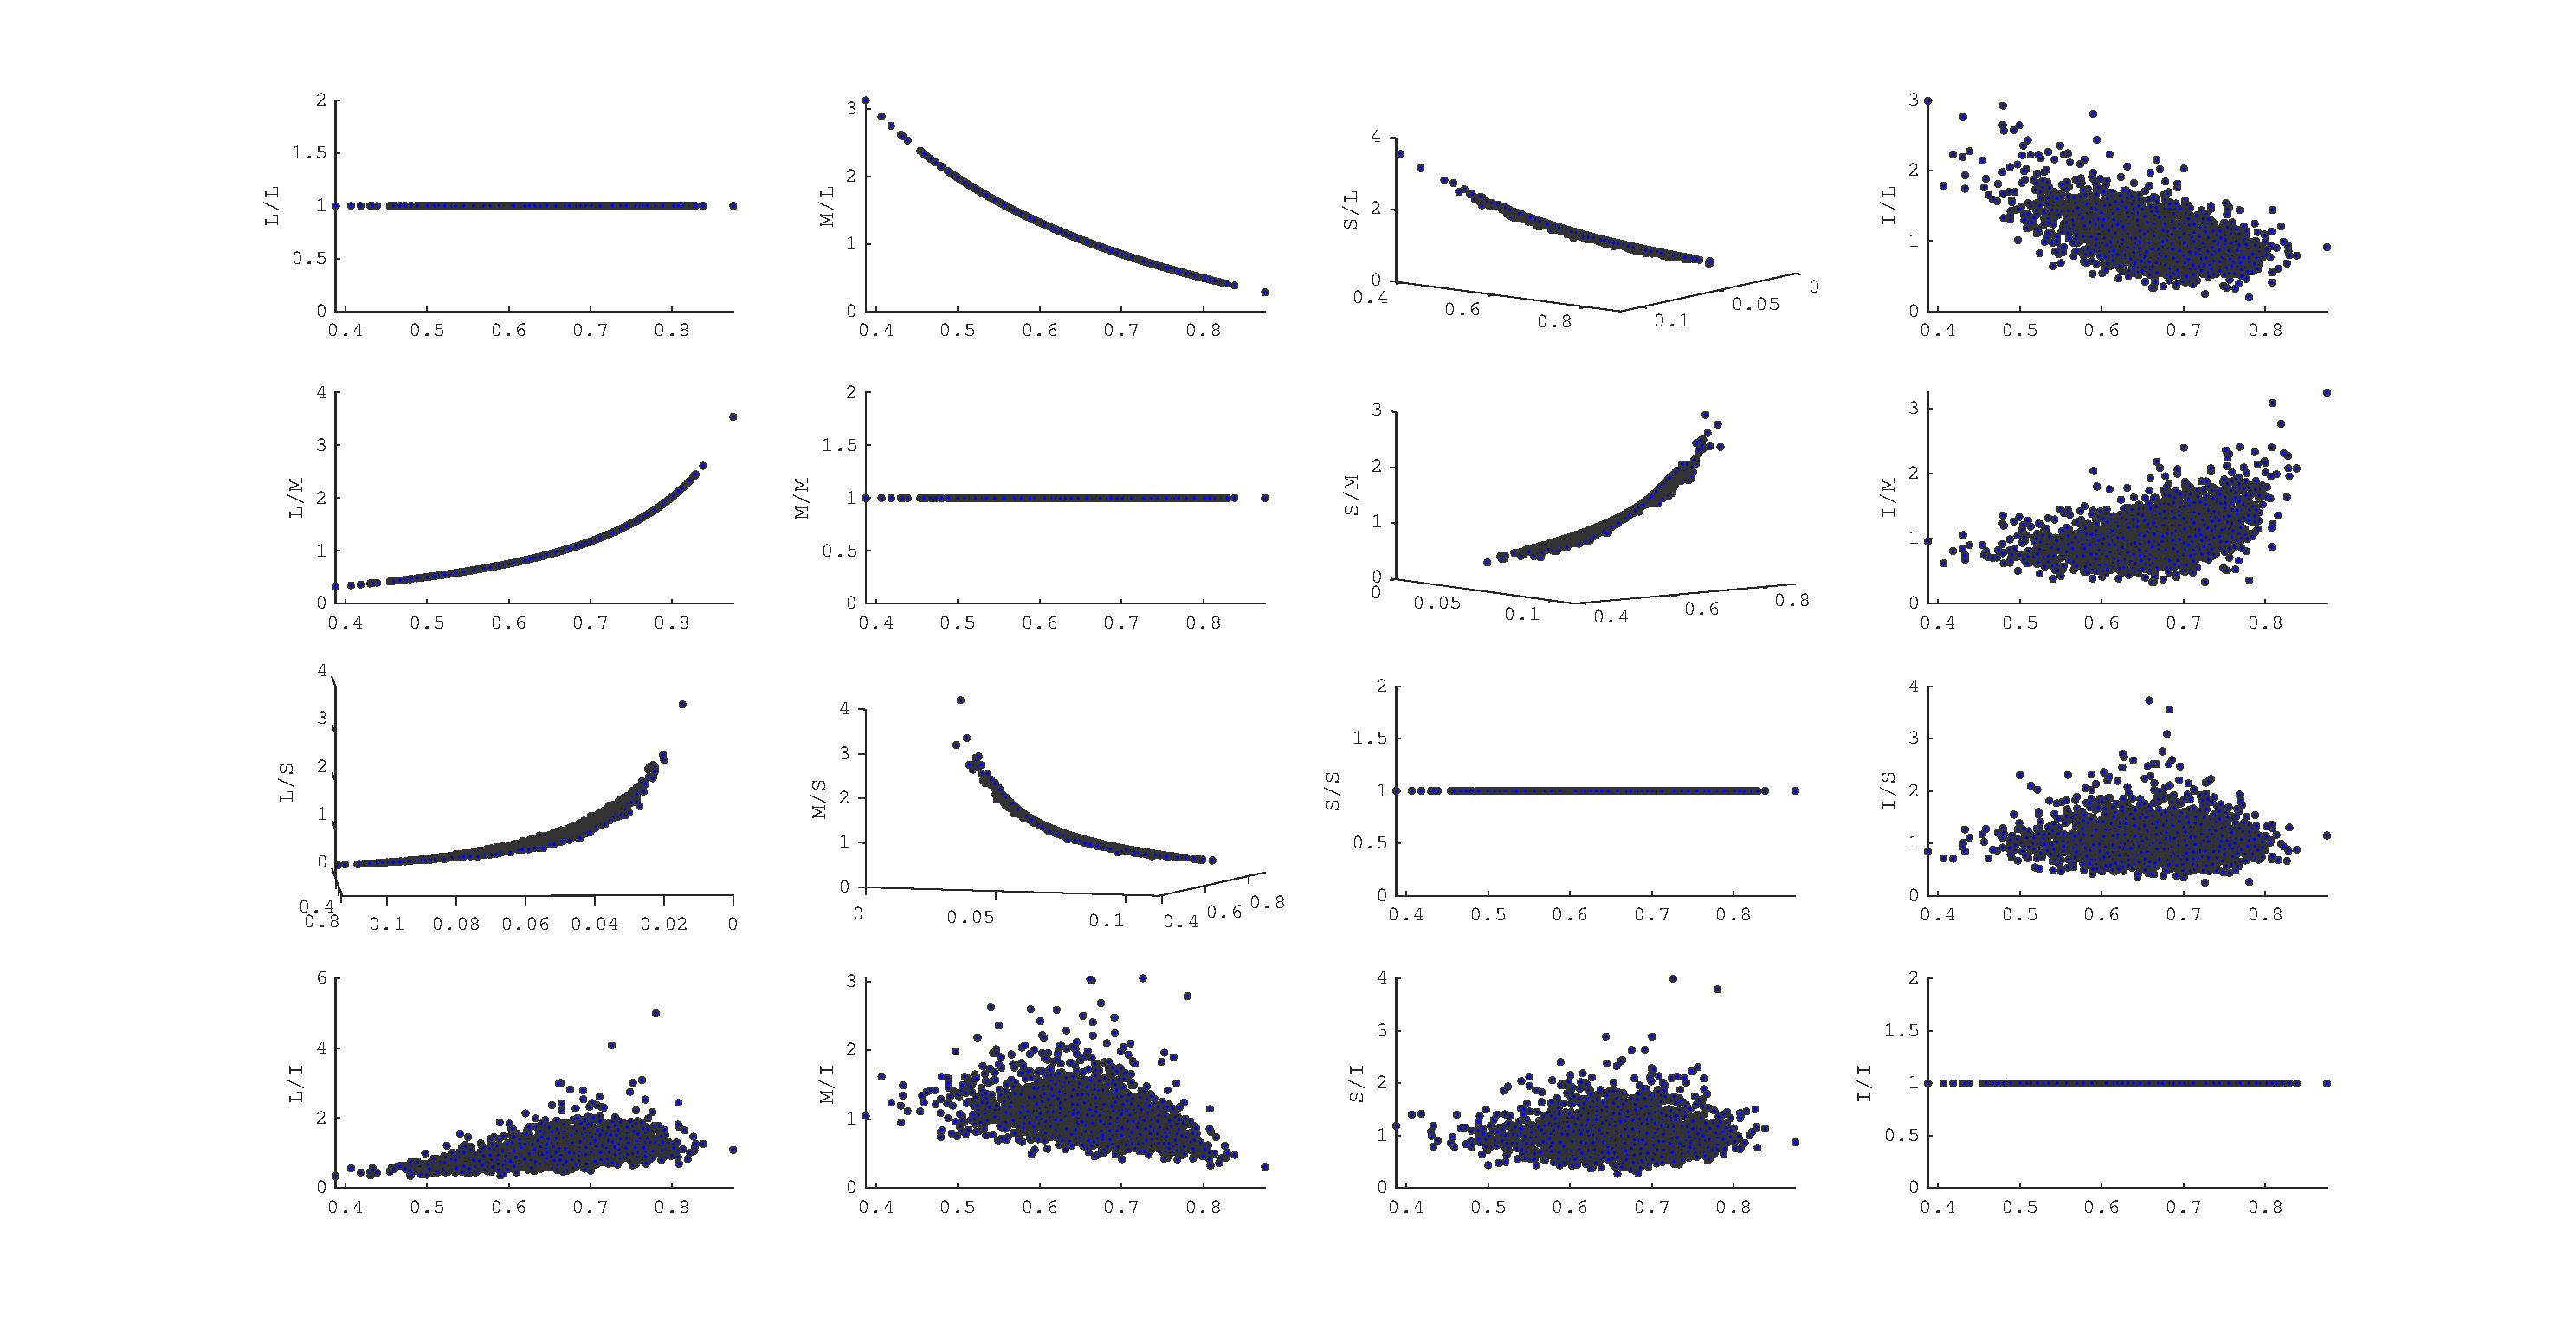
\includepdf[pages=-,rotate=90, offset=75 -75]{figs/comp/melcomp_1/allComboSignals_rand.pdf}
\begin{figure}[h!]
    \caption{As per \ref{fig:allComboSignals} but where $[L,M,S,I]$ was replaced by randomly generated values, and the second level signals were generated from these instead of real values. Where relationships still exist, this implies that they are computational artefacts rather than underlying relationships. Blue is used to distinguish this random data from previous real data.}
    \label{fig:allComboSignals_rand}
\end{figure} 
%\clearpage
% does it look weird if this doesn't spread over a double?

This example shows that if a melanopic signal exhibits correlation with a chromatic signal \emph{not} due to the underlying mathematics of how chromaticity is calculated, and that any relationship must follow from a genuine regularity in the data.

Considering my second question more closely, rather than just looking for a correlation with chromaticity, I considered whether it was possible to perform a conversion of the computed surface chromaticities into an abstract illuminant-independent space, using a melanopic value as a corrective signal. Having seen that the absolute melanopic values seemed to offer little predictive benefit (see Figure \ref{fig:level1}) I chose to create a normalised melanopic value similar in nature to the MB values. Following equation X % 
but with a melanopic value in place of the $S$ value allowed for the creation of what I shall term the $i_{\text{MB}}$ values.

It was found through an optimisation procedure that through addition and subtraction of weighted $i_{\text{MB}}$ values, using the scaling factors shown in equation \ref{eq:correction} such a conversion could approximately be performed. The optimisation sought optimal weights for the scaling factors with the goal of minimising the overall spread of chromaticities (measured as standard deviation of the entire set\footnote{Spoiler: this was a bad idea.}). The effect of different weights can be seen in Figure \ref{fig:minSD}. The results of applying equation \ref{eq:correction} can be seen in figure \ref{fig:corrected}.

\begin{subequations} \label{eq:correction}
\begin{align}
l_{\text{MB}}* &= l_{\text{MB}} + 0.30i_{\text{MB}}\\ %these will have changed
s_{\text{MB}}* &= s_{\text{MB}} - 0.21i_{\text{MB}}
\end{align}
\end{subequations}

\begin{figure}[htbp]
    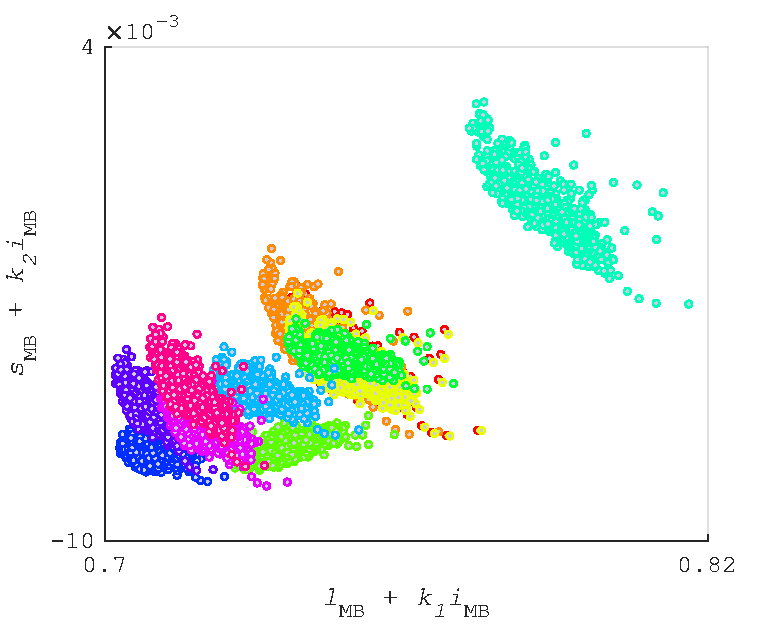
\includegraphics[max width=\textwidth]{figs/comp/melcomp_1/correctedChromaticities.pdf}
    \caption{\gls{MB} chromaticities for 12 reflectances under 2600 daylight illuminants, corrected by the corresponding $i_{\text{MB}}$ value.}
    \label{fig:corrected}
\end{figure} 

It can be seen that the points now roughly cluster together by object, with less smearing induced by changes in illuminant.

Following this, a further optimisation procedure was performed, to consider whether shifting the sensitivity of the melanopsin function along the wavelength spectrum affected the performance of such a signal. Each new sensitivity function was allowed the benefit of the first type of optimisation, allowing different scaling factor weights. The results of this optimisation can be seen in figure \ref{fig:opt}. It can be seen that minima for $l_{\text{MB}}$* occur at around 530nm and just under 600nm, and minima for $s_{\text{MB}}$* occur at around 450nm and 580nm. On first appearance this seems to suggest that the optimal spectral sensitivity for a cone type employed to correct the signals from the various cones might be around these points in the spectrum. However, the careful reader might note the correspondence between the figures above and the peak spectral sensitivities of the cones themselves (S-448nm, M-541nm, L-569nm). Indeed we see that the optimal performance occurs when the nominal melanopsin sensitivity overlaps most well with the spectral sensitivity of the cones. It is understandable why this occurs - each signal is then normalised by a near-duplicate of itself, rendering each value in the set being close to zero. Since we set the goal of the optimisation procedure to be the reduction of the standard deviation of the \emph{entire set}, the optimisation finds these near-duplicate values to be very effective.

\begin{figure}[htbp]
    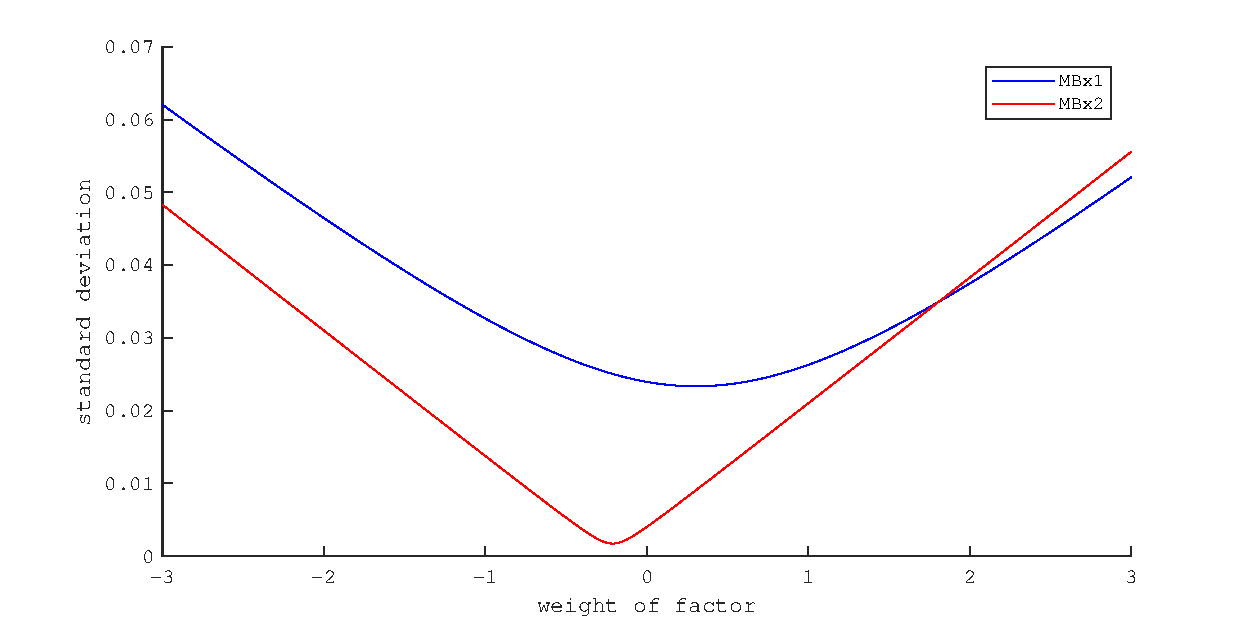
\includegraphics[max width=\textwidth]{figs/comp/melcomp_1/minimiseSD.pdf}
    \caption{A plot showing the optimal minima for the factor weights.}
    \label{fig:minSD}
\end{figure} 

\begin{figure}[ht]
    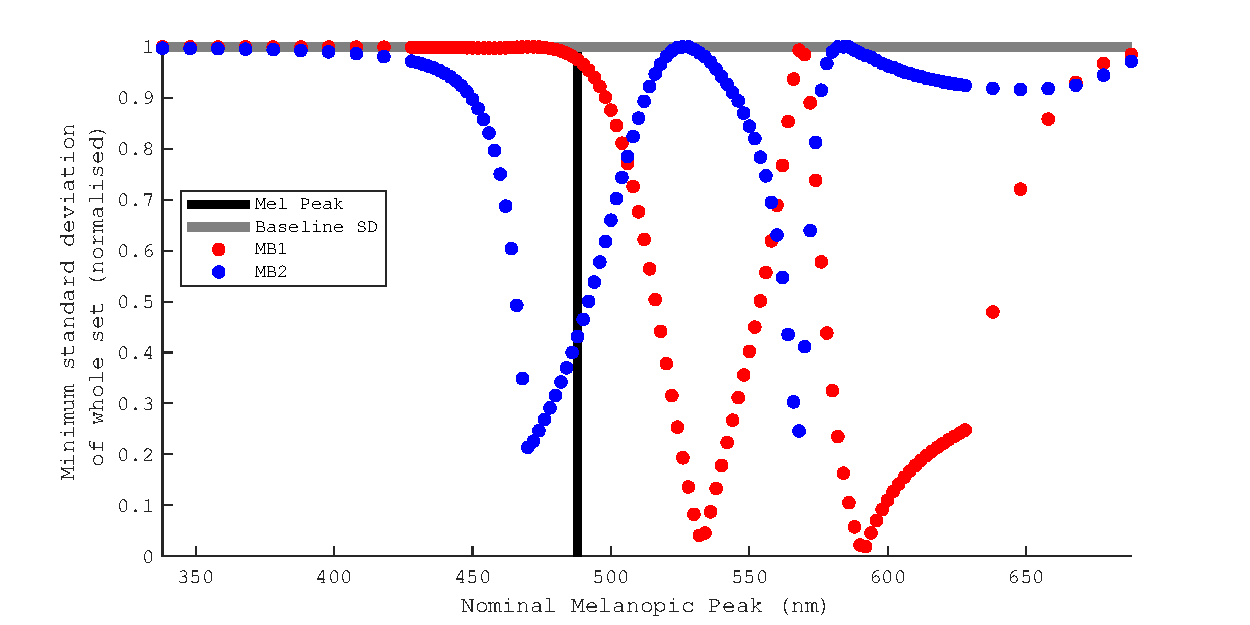
\includegraphics[max width=\textwidth]{figs/comp/melcomp_1_caller/opt.pdf}
    \caption{The results of an optimization where the spectral sensitivity of the nominal melanopsin fundamental was shifted along the spectrum. Generated using melcomp\_1\_caller.m for iteration.}
    \label{fig:opt}
\end{figure} 

Using these values had the unexpected and unfortunate effect of simply crushing all the chromaticties down onto a single line, without preserving any inter-object chromatic differences. We witness perfect colour constancy, at the expense of any chromatic discrimination\footnote{At my poster at VSS David Brainard referred to this as the 'Ford Model of Colour Constancy' - you can have any colour, so long as it's black}. This is obviously not ideal.

\begin{figure}[htbp]
    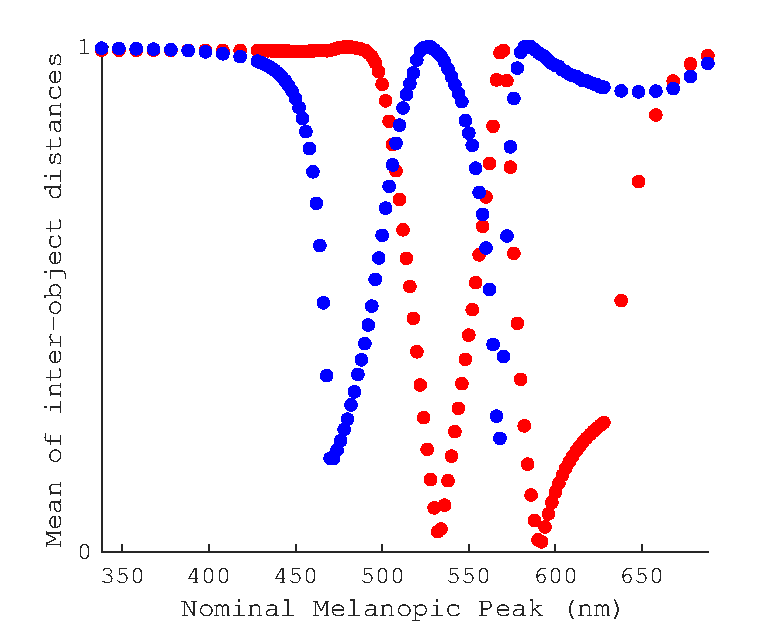
\includegraphics[max width=\textwidth]{figs/comp/melcomp_1_caller/sdmeans.pdf}
    \caption{Normalised average distance between points in the set of the mean chromaticities for the different reflectances. It can be seen that inter-reflectance variation drops to zero at the same minima as seen in figure \ref{fig:opt}, showing that these distinct points are undesirably corrected to the same point. Generated using melcomp\_1\_caller.m for iteration.}
    \label{fig:sdmeans}
\end{figure} 

\textit{The work was presented at this stage as a poster at the \emph{Vision Science Society Conference (VSS)} in 2018.}

The actual desired behaviour would be to minimise internal variance for each reflectance group, whilst maintaining at least some distinction between inter-reflectance groups. A comprehensive approach to this question would need to consider the relative importance of the two separate requirements, and apply appropriate weightings.

To summarise melcomp\_1, and address the questions laid out at the start:
\begin{enumerate}
    \item A basic melanopic signal, computed from direct daylight measurements, cannot predict chromaticity, other than a crude estimation of whether a measurement is direct sunlight or not. \emph{Figure \ref{fig:level1}}
    \item The same can be said for melanopic values computed for daylight reflected off a surface. \emph{Figure \ref{fig:level1}}
    \item A first level melanopic value is highly correlated with first level cone signals. \emph{Figure \ref{fig:tristimCorrelation}}
    \item There are relatively strong relationships between hypothetical second level signals (\emph{Figure \ref{fig:allComboSignals}}) but some of these appear to be nothing more than computational artefacts (\emph{Figure \ref{fig:allComboSignals_rand}}). Notably, the melanopic second level signals did not suffer in this way.
    \item A basic corrective procedure was applied, which seemed to reduce the spread of chromaticities. \emph{Figure \ref{fig:corrected}} 
    \item It was found that when the melanopic value was replaced by signals generated from different spectral sensitivities, and passed through the same optimisation procedure, the best performing signals were near-duplicates of existing signals. These signals performed very well judged by our metric of entire set standard deviation, but in practice would make very poor corrective signals. \emph{Figure \ref{fig:sdmeans}}
    \item I did not reach the stage of considering which objects/luminance levels/daylight chromaticities a melanopic signal might be best/worst suited for. Further development required.
\end{enumerate}
